\chapter{Operation Modes}
The Operation Modes section defines specific modes of the system, such that the system will operate differently during each mode.

Figure~\ref{useCase} shows the list of operation modes that we wanted the final product to have, but due to time constraints we only implemented the "Reading" mode.

\begin{figure}
	
	\centering
	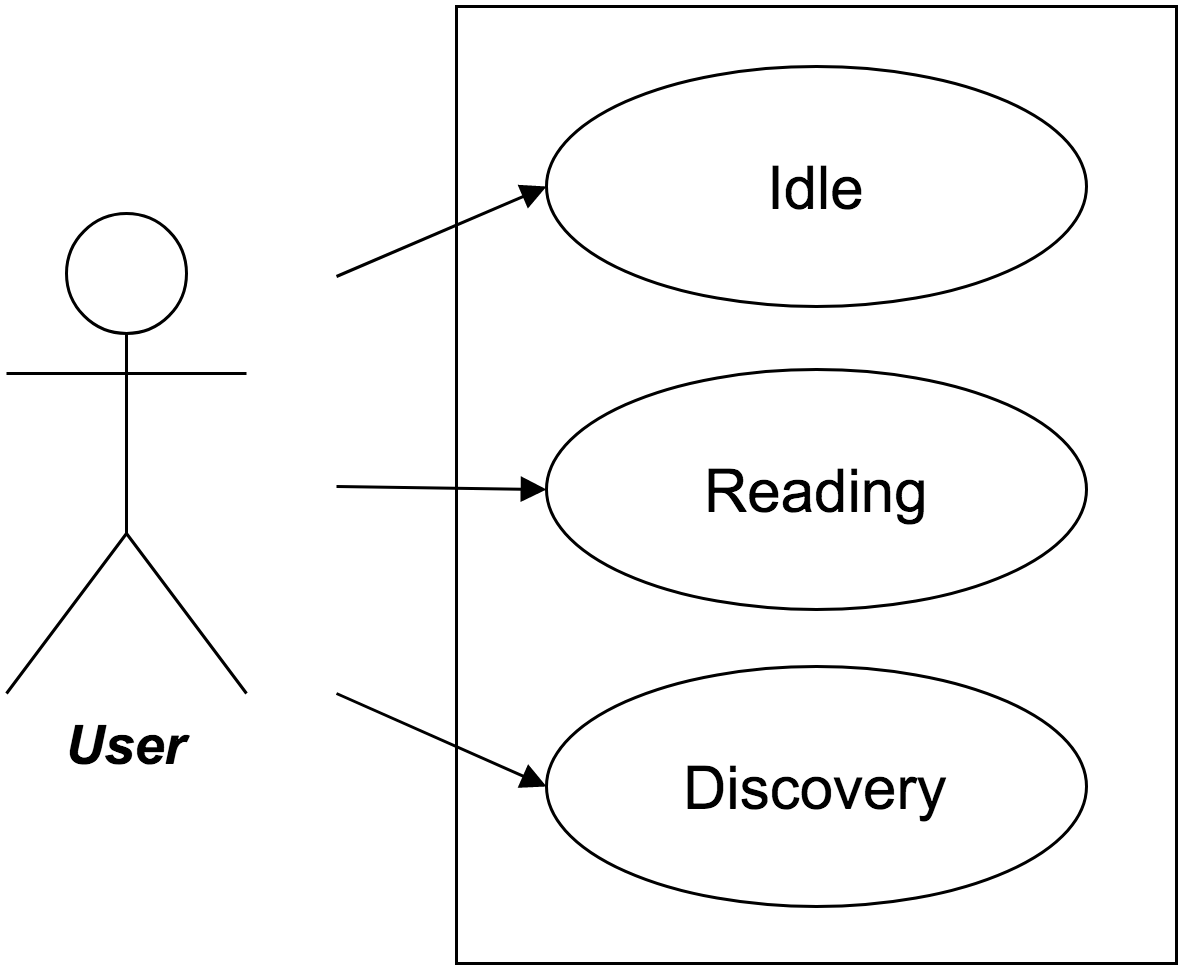
\includegraphics[scale = 0.15]{useCase.png}
    
    \caption{Operation Modes}
    \label{useCase}
\end{figure}

\pagebreak

\section{Idle}
During the Idle mode, the device is put to sleep, this can be done when the user locks the smart phone. By doing so, the power supply of the device can be conserved when it is not using.

\section{Reading}
Reading mode is designed for situations where the user is sitting down or looking at a fixed location. Where the user is desire to "read" the document in front of him or her. During this mode, the device knows the user is looking at the document of interest, thus it can identify and provide the user with detailed information of the document.

\section{Discovery}
Discovery mode is intended for user to explore around the environment, it will provide the user with basic information when the device identifies them.

\begin{table}[]
\centering
\caption{Operation Mode Properties}
\label{Operation_Mode_Properties}
\begin{tabular}{|l|l|l|l|}
\hline
                        & \multicolumn{1}{c|}{\textbf{Idle}}                                                    & \multicolumn{1}{c|}{\textbf{Reading}}                                                                               & \multicolumn{1}{c|}{\textbf{Discovery}}                                                                           \\ \hline
\textbf{Goal}           & \begin{tabular}[c]{@{}l@{}}Put the device to \\ sleep to preserve power\end{tabular}  & \begin{tabular}[c]{@{}l@{}}Identify and obtain large\\ amount of text and provide\\ feedback to user\end{tabular}   & \begin{tabular}[c]{@{}l@{}}Inform the user about\\ potential point of\\ interest around him\\ or her\end{tabular} \\ \hline
\textbf{Actor}          & \multicolumn{3}{c|}{User}                                                                                                                                                                                                                                                                                                       \\ \hline
\textbf{Preconditions}  & \begin{tabular}[c]{@{}l@{}}Device must be turned\\ on\end{tabular}                    & \begin{tabular}[c]{@{}l@{}}Device must be turned on\\ and set to Reading Mode\end{tabular}                          & \begin{tabular}[c]{@{}l@{}}Device must be turned\\ on and set to Discovery\\ Mode\end{tabular}                    \\ \hline
\textbf{Steps}          & \begin{tabular}[c]{@{}l@{}}User set the \\ device to idle\end{tabular}                & \begin{tabular}[c]{@{}l@{}}User stares at the document\\ and directs the device to\\ capture the image\end{tabular} & \begin{tabular}[c]{@{}l@{}}User needs to move his\\ or her head around to\\ capture the surroundings\end{tabular} \\ \hline
\textbf{Postconditions} & \begin{tabular}[c]{@{}l@{}}Disconnect connection\\ to headset and server\end{tabular} & Audio feedback send to user                                                                                         & \begin{tabular}[c]{@{}l@{}}Audio feedback sent\\ to user\end{tabular}                                             \\ \hline
\textbf{Exceptions}     & \multicolumn{1}{c|}{N/A}                                                              & \multicolumn{2}{l|}{\begin{tabular}[c]{@{}l@{}}Unstable input, such that the motion of the headset is\\ outside the threshold\end{tabular}}                                                                                             \\ \hline
\end{tabular}
\end{table}